\documentclass[11pt]{article}
\usepackage{hyperref}
\usepackage{subfigure}

\usepackage[margin=1in]{geometry}

\usepackage{hyperref}
\hypersetup{unicode=true, colorlinks, breaklinks, citecolor=blue, linkcolor=black}

\usepackage{xltxtra}
\usepackage{booktabs} 
\usepackage{subfigure}
\usepackage{graphicx}

\title{Data Mining Capstone Task 2}
%\author{Jiacheng Pan}

\begin{document}
\maketitle

\section{Abstract}

\section{Implementations}
\subsection{Task 2.1: Visualization of the Cuisine Map}
In this sub-task, I manually selected the categories (cuisines) with names indicating cuisines of certain region of the globe (e.g. American\_New, Chinese, etc.), among the top-100 categories with most reviews, to perform the similarity analysis.
Essentially, for each category, I concatenated all its reviews, and computed the similarities between categories based on the similarities of those concatenated review corpuses.

\vspace{1em}
Figure \ref{fig:text_repr} shows the similarity matrix using a matrix diagram.

The opacity level indicates how similar the categories are -- the darker the more similar.

\begin{figure}[htp!]
  \centering
  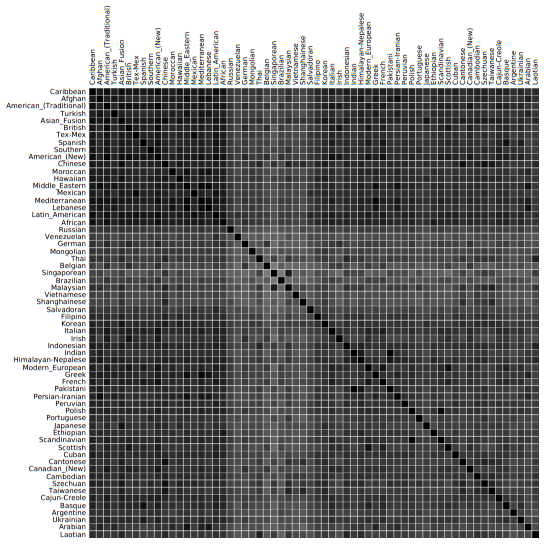
\includegraphics[width=0.6\textwidth]{./img/text_repr.png}
  \caption{Similarity matrix computed based on plain review texts}
  \label{fig:text_repr}
\end{figure}


In this computation, only stop-word removal and normalisation was performed.
Based on the result shown, it is hard to tell which cuisines are more similar than others -- it looks they are very similar to each other, of almostly the same similarity level.

\subsection{Task 2.2: Improving the Cuisine Map}
\subsubsection{Using TF-IDF to improve the cuisine map}
In this sub-task, using the same database (cuisines of regions), and still using text representation of all reviews, I applied
\begin{enumerate}
    \item sublinear TF modifier to penalise high-frequency terms in the same cuisine;
    \item IDF to penalise common terms amongst all documents (cuisines).
\end{enumerate}


\vspace{1em}
Figure \ref{fig:text_repr_tf_idf} shows the similarity using a matrix diagram.

Figure \ref{fig:text_repr_tf_idf_cluster} shows the same matrix, while applying K-mean clustering method to cluster the cuisines into three clusters.

The order of cuisines has been sorted by the closeness between each other.

\begin{figure}[htp!]
  \centering
  \subfigure[Without cluster] {
    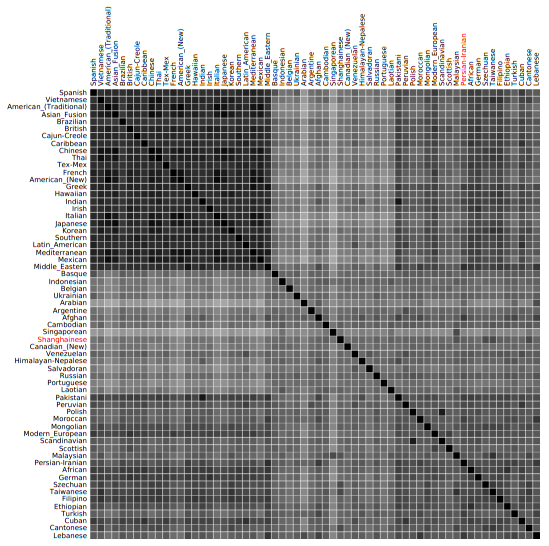
\includegraphics[width=0.6\textwidth]{./img/text_repr_tf_idf.png}
    \label{fig:text_repr_tf_idf}
  }
  \subfigure[With cluster] {
    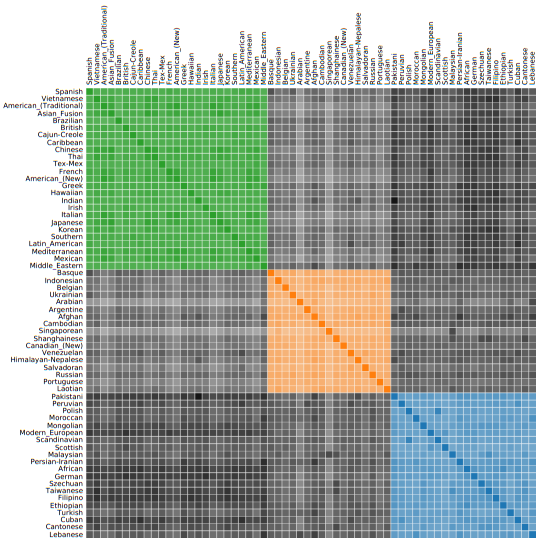
\includegraphics[width=0.6\textwidth]{./img/text_repr_tf_idf_cluster.png}
    \label{fig:text_repr_tf_idf_cluster}
  }
  \caption{Similarity matrix computed based on plain review texts, with TF-IDF modifiers}
\end{figure}


As is shown, the diversity of similarity has been improved (to be more diversed), so that it is clearer to see which cuisines are similar to each other.

Actually, as is depicted, there are roughly three major clusters --
\begin{enumerate}
    \item the top: darkest, showing that between these cuisines, they are highly similar to each other;
    \item the middle: lightest, showing these cuisines are possibly peripherial ones;
    \item the bottom: intermediate but lighter for intra-cluster, but darker for inter-cluster with the top cluster, showing these cuisines are between the outer peripherial cuisines and the inner core cuisines.
\end{enumerate}

Let's do a brief analysis on why applying TF-IDF can improve the diversity:

Without TF-IDF, common words among all the cuisines are taken into consideration. These common words are common in the sampled corpuses, while may not be as common in the English language or other corpuses. So they cannot be removed by stop words, and they do a lot of harm to the diversity because between cuisines, these words are usually shown, contributing to higher similarity in this approach, which computes the similarity based on the plain text representations.

\subsubsection{Using LDA to improve the cuisine map}
Here I not only applied TF-IDF modifiers, but also applied LDA to mine the topics of each cuisine, and compute the similarity based on the term distribution of the topics of each cluster.

The amount of topics I specified is 100.

\vspace{1em}
Figure \ref{fig:topic_tf_idf} shows the similarity using a matrix diagram.

Figure \ref{fig:topic_tf_idf_cluster} shows same matrix, while clustered by KMeans.

\begin{figure}[htp!]
  \centering
  \subfigure[Without cluster] {
    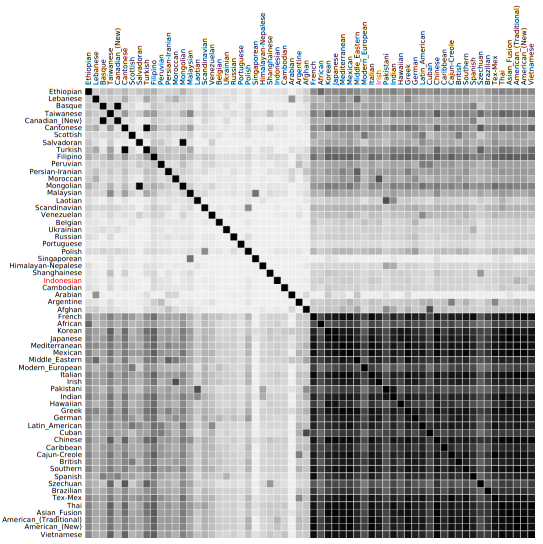
\includegraphics[width=0.6\textwidth]{./img/topic_tf_idf.png}
    \label{fig:topic_tf_idf}
  }
  \subfigure[With cluster] {
    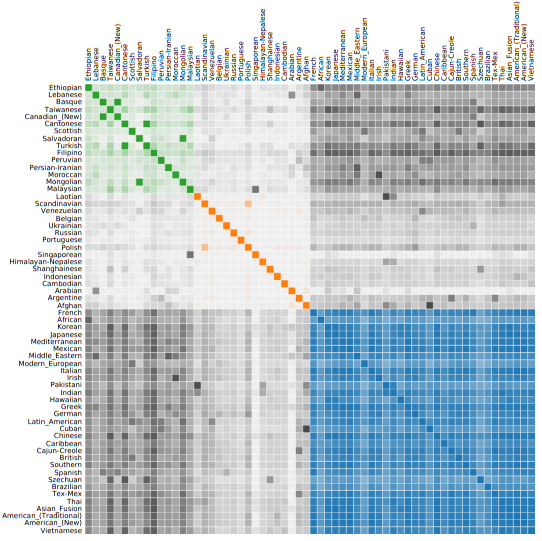
\includegraphics[width=0.6\textwidth]{./img/topic_tf_idf_cluster.png}
    \label{fig:topic_tf_idf_cluster}
  }
  \caption{Similarity matrix computed based on topics mined with LDA and TF-IDF modifiers}
\end{figure}

\begin{figure}[htp!]
  \centering
  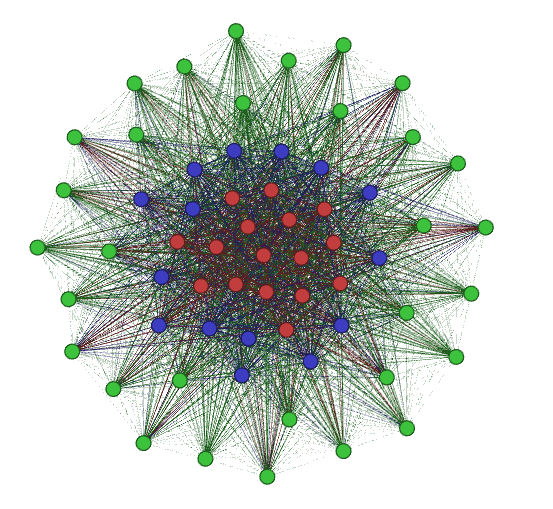
\includegraphics[width=0.6\textwidth]{./img/topic_tf_idf_force_layout.png}
  \label{fig:topic_tf_idf_force_layout}
  \caption{Force Atlas layout in Gephi, plotting the similarity matrix computed by LDA and TF-IDF, nodes coloured based on the clustering result computed by KMeans}
\end{figure}


It is even more obvious that three clusters can be identified -- the inner, the outer, and the intermediate.
\vspace{1em}

To better visualise the result, I used software Gephi to plot a Force-Atlas layout, using cuisines as the nodes, and the similarities as the link weights.

Figure \ref{fig:topic_tf_idf_force_layout} shows the result. The nodes are coloured to indicate which groups they belong to, according to the KMeans result.

\vspace{1em}

To analyse why using LDA can improve the diversity between cuisines:

We can see that LDA is actually a dimensionality-reduction method.
By using it, we actually are reducing the dimension of the entire dataset, from the size of all the vocabularies, into the size of all topics (which is 100).
If doing correctly, dataset of lower-dimension is much denser, therefore is less susceptible to the noises caused by high dimensionality.

Therefore, it is easier to produce a more diversed similarity matrix, to show a clearer picture of how cuisines are related.


\subsection{Task 2.3: Incorporating Clustering in Cuisine Map}
\subsubsection{Using KMeans}

In this sub-task, I applied K-means method to do the clustering, based on the similarity matrix computed using LDA and TF-IDF modifiers.

\vspace{1em}
Figure \ref{fig:cluster_3}, \ref{fig:cluster_6}, and \ref{fig:cluster_9} show the result of clustering the matrix into three, six, and nine sized clusters

The coloured cells indicate that both of the cuisines are of the same cluster, and vise versa.

\begin{figure}[htp!]
  \centering
  \subfigure[Size 3] {
    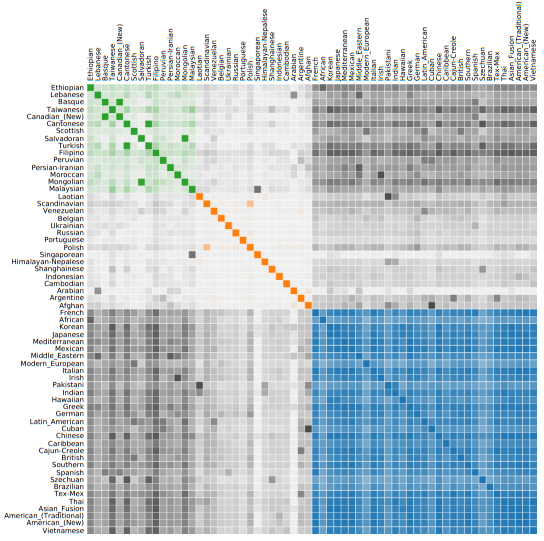
\includegraphics[width=0.6\textwidth]{./img/cluster_3.png}
    \label{fig:cluster_3}
  }
  \subfigure[Size 6] {
    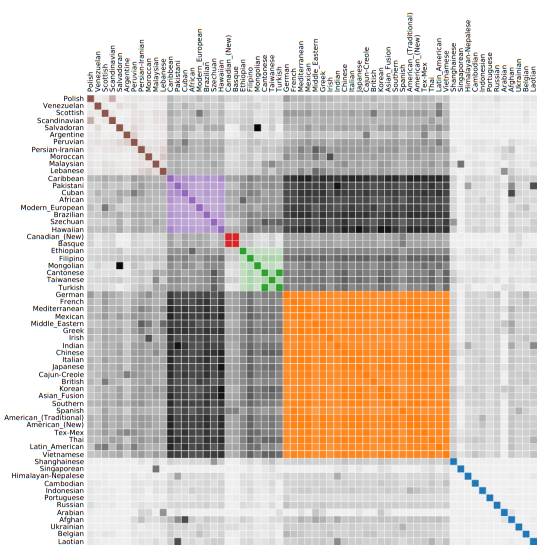
\includegraphics[width=0.45\textwidth]{./img/cluster_6.png}
    \label{fig:cluster_6}
  }
  \subfigure[Size 9] {
    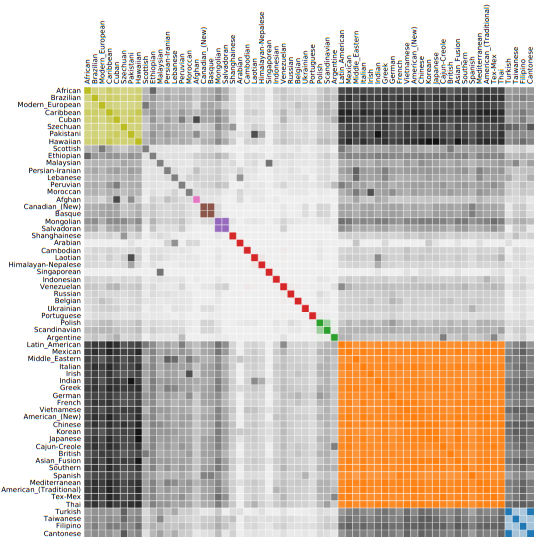
\includegraphics[width=0.45\textwidth]{./img/cluster_9.png}
    \label{fig:cluster_9}
  }
  \caption{Clustering using KMeans, on the similarity matrix computed based on topics mined with LDA and TF-IDF modifiers}
\end{figure}

\vspace{1em}
As is shown, the 3-cluster result is closest to the matrix characteristics -- inner, outter, and intermediate.
In fact, this clustering result is relatively more balanced.

However, for the 6-cluster, although the sizes of most of the clusters are similar, the inter-cluster closeness is compromised -- 
As we can see from the orange and purple clusters, their similarities across clusters are very high, indicating they should have been clustered as one, further indicating the number of clusters specified is too high.

So we can see that the 6-cluster result is less useful than the 3-cluster one.

As for the 9-cluster result, it is even worse --
\begin{enumerate}
  \item the sizes of clusters are skewed (there is one 1-sized cluster, two 2-sized, one 3-sized and 4-sized clusters, compared to the huge orange, red and yellow clusters);
  \item the yellow and orange clusters are high in terms of inter-cluster similarity.
\end{enumerate}

\vspace{1em}
Therefore, we can conclude that for this particular similarity matrix, it is more meaningful to examine the 3-cluster result, while clustering into higher number of clusters is less useful.

\subsubsection{Using Agglomerative Clustering}
I also tried agglomerative clustering method to do the clustering.

Figure \ref{fig:hier_cluster_3} and \ref{fig:hier_cluster_3_force} show the results in matrix diagram and force layout, using the same database as the KMeans used, i.e. similarity computed based on LDA and TF-IDF.

It turns out that in this specific case, both of the methods yield similar results.

To analyse, I think possible it is because both of the methods use distance, which here is the similarity, to determine the clusters.


\begin{figure}[htp!]
  \centering
  \subfigure[Matrix Diagram] {
    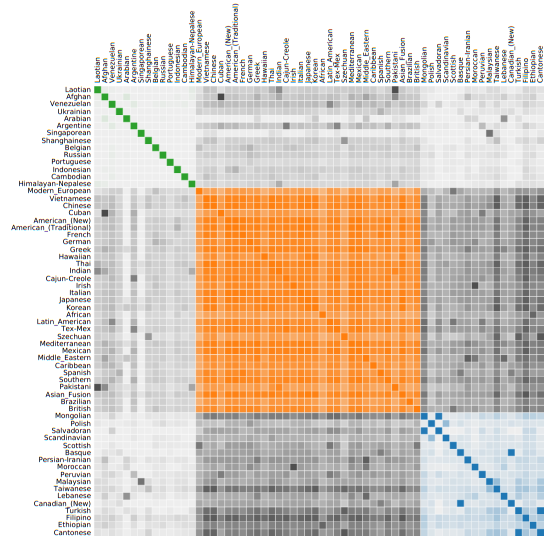
\includegraphics[width=0.6\textwidth]{./img/hier_cluster_3.png}
    \label{fig:hier_cluster_3}
  }
  \subfigure[Force Atlas Layout] {
    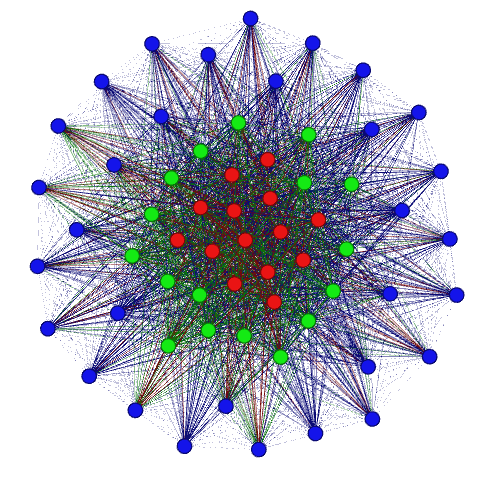
\includegraphics[width=0.45\textwidth]{./img/hier_cluster_3_force.png}
    \label{fig:hier_cluster_3_force}
  }
  \caption{Clustering using Agglomerative Clustering, on the similarity matrix computed based on topics mined with LDA and TF-IDF modifiers}
\end{figure}


\end{document}

